% !Mode:: "TeX:UTF-8"
\documentclass[11pt]{article}
\usepackage[letterpaper, margin = 2cm]{geometry}
\usepackage{microtype}
\usepackage{parskip}
\usepackage{amssymb}
\usepackage{amsmath}
\usepackage{multicol}
\usepackage{graphicx}
\usepackage{booktabs}
\usepackage{caption}
\usepackage{float}
\usepackage[style=ieee]{biblatex}
\usepackage[bookmarks, unicode]{hyperref}

\addbibresource{references.bib}

\title{Heat Flux}
\author{Josh Kraan}
\date{\today}

\begin{document}

\maketitle

\section{Gas Properties}

%TODO future or past tense??

Combustion gas properties are commonly calculated using NASA's Chemical Equilibrium with Applications (CEA) \cite{} program, however this FORTRAN program is difficult to work with. Instead the combustion gas properties were calculated using Cantera as described by Youngblood \cite{}.

Species included in the chemical equilibrium calculations were based off of those used in CEA and kerosene combustion models \cite{} as well as the availability of tranport properties. The species that were included in this analysis are: RP-1, LOX, CO, CO2, H, H2, H2O, O, OH, and O2. RP-1 and LOX were modelled with the same stoichiometry and heat of formation as used in CEA. Cantera requires transport parameters for all species, so RP-1 and LOX were assigned placeholder values with the understanding that equilibirum solutions contain essentially zero concentration of these species.

Thermodynamic properties and Lennard-Jones transport parameters were taken from a high-temperature version of the GRI MECH 3.0 combustion mechanism \cite{} included with Cantera that has been extended from an upper temperature of 3500K to 6000K using thermodynamic properties from NASA \cite{}.

\subsection{Property Evaluation}

The stagnation pressure is found by solving

\begin{equation}
  \dot{m} = p_0 A_t \sqrt{\frac{\gamma [2 / (\gamma + 1)]^{\frac{\gamma + 1}{\gamma - 1}}}{R_{gas} T_o}}
\end{equation}

The stagnation gas properties at each pressure are calculated using the same method as described by Youngblood.

Two nested root finders were used to calculate gas properties throughout the converging-diverging sections of the engine. The outer root finder solves the isentropic flow relation for pressure: %TODO cite

\begin{equation}
  \frac{p}{p_0} = (1 + \frac{\gamma - 1}{2} M^2) ^ {- \frac{\gamma}{\gamma - 1}}
\end{equation}

The specific heat ratio for the combustion gas is calculated at each evaluated pressure and the chamber entropy. The specifc heat ratio and the area ratio are used to solve the mach number equation using the other root finder. Subsonic or supersonic solutions are forced by changing the bracketing interval depending on axial location.

\begin{equation}
    \left( \frac{A}{A_t}\right)^2 = \frac{1}{M^2} \left\{ \frac{2}{\gamma + 1} \left[ 1 + \frac{1}{2} (\gamma - 1) M^2 \right] \right\}^{\frac{\gamma + 1}{\gamma - 1}}
\end{equation}

Despite requiring nested root finders, this method was found to perform better than solving the pressure-area ratio relations.

With the pressure and entropy known, all other gas properties can be calculated. The gas velocity is calculated from the mach number and the local speed of sound:

\begin{equation}
  v = M \sqrt{\gamma p / \rho}
\end{equation}

\subsection{Frozen Boundary Layer Chemistry}

CEA calculates ``frozen'' and ``equilibrium'' values for specific heat and thermal conductivity. Equilibrium values are taken to be the sum of the frozen value and a reaction term that accounts for chemical reactions occuring in the boundary layer. Equilibirum values for both are several times higher than frozen, and using the equilibrium values would lead to a calculated heat flux approximately 4.5 times higher (based on the Bartz equation).

Bartz \cite{page 46} discusses chemical reactions occuring in rocket engine boundary layers and the resulting increase in heat transfer. When dissociated species such as O, H, and OH are present in the free stream, they can cool against combustion walls and recombine exothermically in the boundary layer. Bartz notes that this effect would likely be maximum for a hydrogen and oxygen rocket at 100\% combustion efficiency, yet the increase in heat flux over a frozen layer is shown to be only 32\% and rapidly decreases with reduced combustion efficiency.

The presence of dissociated species is not insigificant for this engine, as can be seen in figure \ref{}. It is unclear why equilibirum values calculated by CEA are so high and reproducing them is difficult, so based off of the Bartz information the boundary layer was considered to be chemically frozen.


\begin{minipage}{.5\linewidth}
  \centering
  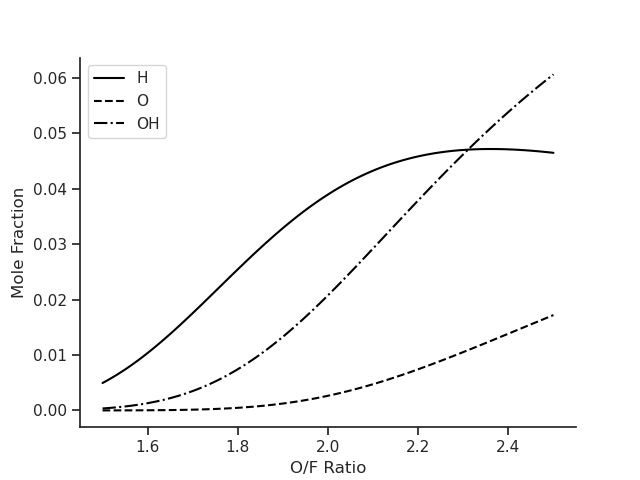
\includegraphics[width=\linewidth]{dissociated-chamber.png}
  \captionof{figure}{Chamber dissociated species.}
\end{minipage}%
\begin{minipage}{.5\linewidth}
  \centering
  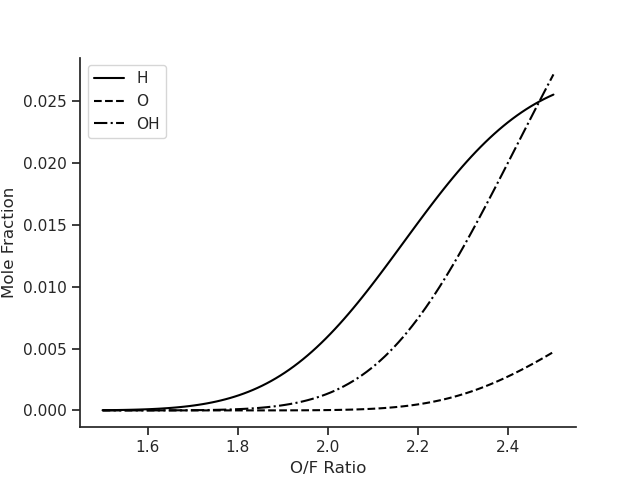
\includegraphics[width=\linewidth]{dissociated-nozzle.png}
  \captionof{figure}{Nozzle dissociated species.}
\end{minipage}

\subsection{Frozen Contraction and Expansion}

Through the contraction and expansion of the engine, combustion gas can be considered to either be in equilibrium (mole fractions change along length of engine) or the composition could be frozen. Both methods were implemented, but this was found to make little difference to heat flux calculations.

%TODO look into more

\subsection{Property Comparison}

\begin{table}[H]
  \centering
  \caption{Cantera and CEA property comparison, OF = 2.29.}
  \begin{tabular}{l c c c c c c}
    \toprule
    & \multicolumn{2}{c}{Stagnation} & \multicolumn{2}{c}{Throat} & \multicolumn{2}{c}{Exit} \\
    \cmidrule(lr){2-3} \cmidrule(lr){4-5} \cmidrule(lr){6-7}
    & Cantera & CEA Diff. & Cantera & CEA Diff. & Cantera & CEA Diff. \\
    \midrule
    T (K) & 3307.3 & $-0.09\%$ & 3135.7 & $0.23\%$ & 2660.9 & $1.16\%$ \\
    $C_p$ ($10^3$ J/kg/K) & 2.0766 & $-0.05\%$ & 2.0665 & $-0.04\%$ & 2.0291 & $0.06\%$ \\
    $\rho$ ($10^{-1}$ kg/m$^3$) & 6.2405 & $0.06\%$ & 3.7268 & $3.26\%$ & 0.8617 & $10.5\%$\\
    $\gamma$ & 1.2256 & $-4.09\%$ & 1.2228 & $-4.63\%$ & 1.2185 & $-5.23\%$ \\
    $\mu$ ($10^{-5}$ Pa s) & 9.4636 & $8.03\%$ & 9.1093 & $8.42\%$ & 8.0947 & $9.60\%$ \\
    $k$ ($10^{-1}$ W/m/K) & 3.5662 & $-3.87\%$ & 3.3775 & $-3.33\%$ & 2.8629 & $-1.72\%$\\
    \bottomrule
  \end{tabular}
\end{table}

All major species were found to have less than 1\% difference in mole fractions between Cantera and CEA throughout the engine. Stagnation thermodynamic properties match very well, which is expected as GRI MECH uses NASA thermodynamic data. Transport properties are consistently different; CEA uses empirical fits but Cantera uses the Lennard-Jones model so this isn't unexpected.

The density and temperature match well at stagnation but diverge from CEA along the length of the engine. This is likely because the specific heat ratios differ. Heat capacity consistently matches with CEA, which is expected as it has low temperature dependence.

\section{Heat Transfer Correlations}

It appears to be accepted to use the difference between the adiabatic wall temperature and the wall temperature as the driving potential for heat flux \cite{}, so that was adopted here as well. The adiabatic wall temperature is given by:

\begin{equation}
    T_{aw} = T + r(T_0 - T)
\end{equation}

The recovery factor $r$ is commonly given as

%TODO temperature to take Pr at?
\begin{equation}
    r = (Pr)^{1/3}
\end{equation}

The gas wall temperature was taken to be a constant value of 500K %TODO

Many models require property evaluation at temperatures other than the free stream temperature. For these models, the gas temperature was changed in Cantera while keeping the pressure constant.

%TODO effect of equilibrium

The largest difference was between the Dittus-Boelter and Bartz models, at 30\%. This was found to be because of the difference in constants (11\%), the throat curvature factor (10\%), and the breakdown of the assumption of constant Prandtl number and specific heat (9\%).

\subsection{Bartz}

%TODO temp dependence of viscosity

The Bartz equation is commonly used for calculating rocket engine heat flux. The following form is common:

\begin{equation}
    \label{equation:bartz}
    \begin{split}
         h_g = \left[ \frac{0.026}{D_t^{0.2}} \left( \frac{\mu^{0.2} c_p}{{Pr}^{0.6}} \right)_{0} \left( \frac{p_0}{c^*} \right)^{0.8} \left( \frac{D_t}{R_c} \right)^{0.1} \right] \left( \frac{A_t}{A} \right)^{0.9} \sigma \\
         \sigma = \frac{1}{\left[ \frac{1}{2} \left( \frac{T_{w}}{T_0} \right) \left( 1 + \frac{\gamma - 1}{2} M^2 \right) + \frac{1}{2}\right]^{0.8-m/5} \left[ 1 + \frac{\gamma - 1}{2} M^2 \right]^{m/5}}
    \end{split}
\end{equation}

$m$ is the exponent of the temperature dependence of viscosity, and it is commonly taken to be 0.6.

This form shows the pressure dependence of heat flux at a constant characteristic velocity, however if the equation is rearranged into nondimensional parameters the fact that it is a modified version of the Dittus-Boelter equation is more clear.

\begin{equation}
  Nu_{t} = 0.026 Re_{t}^{0.8} Pr^{0.4} \left( \frac{D_t}{R_c} \right)^{0.1} \left( \frac{A_t}{A} \right)^{0.9} \sigma
\end{equation}

Here all gas properties are evaluated at stagnation, the throat diameter is the characteristic dimension, and the Reynolds number is evaluated at an effective throat velocity, so

\begin{equation}
  Re_{t} = \frac{D_t (\dot{m} / A_t)}{ \mu_{ns}}
\end{equation}

The $\sigma$ term accounts for property variation in the boundary layer and along the length of the engine.

Another form given by Bartz uses stagnation gas properties but local diameter and velocity. It has a boundary layer property variation term that uses the gas viscosity and density at the arithmetic mean of the free stream and wall temperatures:

\begin{equation}
  Nu_{D} = 0.026 Re_{D}^{0.8} Pr^{0.4} \left( \frac{D_t}{R_c} \right)^{0.1} \left[ \left( \frac{\rho_{am}}{\rho} \right)^{0.8} \left(\frac{\mu_{am}}{\mu} \right)^{0.2}\right]
\end{equation}


\subsection{Dittus-Boelter}

The unmodified Dittus-Boelter equation the Bartz equation is based on is given by:

%TODO just evaluate all properties at mean temp? Film cooling paper
%TODO 0.3 or 0.4?

\begin{equation}
  Nu_{D} = 0.023 Re_{D}^{0.8} Pr^{0.4}
\end{equation}

The Dittus-Boelter equation is known to be ill-suited to modelling flows with large property variations in the boundary layer. A proposed solution is to evaluate all properties at the arithmetic mean of the free stream and wall temperatures \cite{}. Another solution is to evaluate all properties at the reference temperature given by \cite{}:

\begin{equation}
  T_{ref} = 0.5(T + T_w) + 0.22 Pr^{1/3}(T_0 - T)
\end{equation}

\subsection{Sieder-Tate}

\begin{equation}
  Nu_{D} = 0.027 Re_{D}^{0.8} Pr^{1/3} \left( \frac{\mu}{\mu_w} \right)^{0.14}
\end{equation}

\subsection{Colburn}

\begin{equation}
  Nu_x = 0.0296 Re_x^{0.8} Pr^{1/3}
\end{equation}

\begin{equation}
  x_e = 3.53D \left[ 1 + \left( \frac{x}{3.53D} \right)^{-1.2}\right]^{-1/1.2}
\end{equation}

\section{OF Ratio}

\subsection{Constant Pressure}

\subsection{Changing Pressure}

\section{Experimental Data}


\section{Conclusion}

Pintle recirculation zones

Film cooling



\end{document}
